\newpage
\section{Projektaufgabenstellung$^1$}
Die Aufgabenstellung des Projekts ist es einen Webshop für die Firma Global Bike Inc. (folgend GBI) zu erstellen. Diese Firma stellt Fahrräder her und vermarktet diese. Die Produkte des Webshops sollen aus einem ERP-System geladen werden. Bei dem ERP-System handelt es sich um ein schon bestehendes SAP-ERP-System. Alle auf dem Webshop getätigten Bestellungen sollen an das ERP-System weitergereicht werden. Zudem soll für den Benutzer des Webshops der Stand der Bestellung einsehbar sein. Dieser Stand soll ebenfalls aus dem ERP-System übernommen werden. \\
Weitere Kriterien für den Webshop sind, dass dieser in eine APP für mobile Geräte einbindbar sein muss, ein Corporate-Design entworfen werden, sowie ein Marketing-Mix für die Online-Vermarktung im Großraum OWL entwickelt werden soll.

\section{Projektplanung}
Dieser Abschnitt erläutert, wie die Projektplanung dieses Projekts ablief. Es wird der Ablauf, von der Ideenfindung bis durch Planung der Durchführung, erläutert.

\subsection{Ideenfindung$^1$}
Der erste Schritt des Projekts bestand darin zu bestimmen, was für Funktionen der Webshop alles anbieten soll. Hierfür sind drei Onlinewebshops betrachtet worden. Es wurden die Webshops \glqq fahrrad.de\grqq{}, \glqq amazon.de\grqq{} und \glqq alternate.de\grqq{} angeschaut.\\
Vom Webshop \glqq alternate.de\grqq{} ist der Webseitenkopf als sehr sinnvoll empfunden worden. Dieser Kopf ist am oberen Rand der Webseite fest fixiert und wird nicht mitgescrollt. Dieses bietet den Vorteil, dass der Kunde durchgehend die Menge einsehen kann, die sich im Warenkorb befindet. Grund hierfür ist, dass sich eine kleine Warenkorbanzeige mit im Kopf der Webseite befindet. Zudem kann der Benutzer sich durch die Webseite navigieren ohne zu scrollen. Da ebenso im Kopf der Webseite die Suche fixiert ist, kann der Benutzer auch ohne zu scrollen nach etwas suchen. Wegen den vielen Vorteilen wurde beschlossen den Kopf der Webseite weitgehend für den Webshop der GBI zu übernehmen.\\
Aus allen drei Webshops wurde zudem übernommen, dass der Webshop der GBI mit einen Warenkorb gelöst werden soll und die Benutzer sollen Kommentare zu einen Artikel schreiben und lesen können. Ebenso soll es möglich sein, dass der Kunde den Artikel bewerten kann. Der Artikel soll über eine Suche und eine Navigation zugreifbar sein. Zu einen Artikel soll in der Produktbeschreibung mehrere Produktbilder angezeigt werden, die sich der Kunde durch draufklicken größer ansehen kann. Die Produktbeschreibungsseite soll mindestens den Preis, die Bewertung, den Produktnamen und eine ausführlichen Beschreibungstext erhalten.\\
Als negativ wurde empfunden, wenn die Startseite der Webseite \glqq überladen\grqq{} von Produkten ist. Somit wurde beschlossen die Startseite des Webshops übersichtlich zu gestalten.

\newpage
\subsection{Anforderungsanalyse$^2$}
Der zweite Schritt des Projekts war die Anforderungsanalyse. Hier wurde ermittelt, welche Anforderungen genau der Webshop erfüllen muss. Während der Analyse einigte man sich auf folgende Projektanforderungen:
\begin{itemize}
	\item Man sollte sich registrieren können.
	\item Wenn man schon registriert ist, sollte man sich anmelden können.
	\item Die Daten zwischen dem ERP-System und dem Webshop sollen über eine Schnittstellendatenbank ausgetauscht werden.
	\item Um auf mobilen Geräten und Desktop-Computern die Webseite richtig anzeigen zu können soll eine zusätzliche CSS-Datei für mobile Geräte erstellt werden. Diese Datei soll die Style-Anweisungen überschreiben, die vom mobilen Gerät falsch angezeigt werden.
	\item Man sollte ein Artikel über die Navigation und die Suche erreichen.
	\item Die gefundenen Artikel sollten in einen Warenkorb gesammelt werden können (mit Mengenangabe).
	\item Nachdem der Warenkorb gefüllt ist, sollen die Artikel bestellt werden können. Hierbei sollen verschiedene Liefer- und Zahlungsmöglichkeiten auswählbar sein.
	\item Die Bestellung sollte mit einer Bestätigungs-Email bestätigt werden.
	\item Der Zustand der Bestellung sollte nachverfolgbar sein.
	\item Der Kunde sollte den Artikel bewerten können und Kommentare äußern können.
\end{itemize}

\subsection{Geschäftsprozess$^1$}
Als nächstes wurde festgelegt, wie ein Geschäftsprozess beim Webshop aussehen soll. Der Geschäftsprozess beginnt, wenn der Kunde die Webseite aufruft. Darauf folgend registriert sich entweder der Kunde oder er loggt sich mit der vorhandenen Benutzerkennung ein. Danach sucht sich der Kunde Produkte auf der Webseite aus und füllt damit den Warenkorb. Nachdem der Warenkorb gefüllt ist, führt der Kunde die Bestellung durch. Wenn die Firma GBI die  Bestellung erhalten hat, wird an den Kunden eine Bestätigungsmail versendet. Darauf folgend wartet der Webshop auf die Bezahlung der Produkte. Hat die Firma GBI die Zahlung erhalten,  wird die Ware an den Kunden verschickt. \\Dieser Geschäftsprozess ist nochmal in dem als \glqq Business Process Model and Notation\grqq{} dargestellten Geschäftsmodell (\textit{Abbildung 1}) zu sehen.

\begin{figure}[H] 
  \centering
     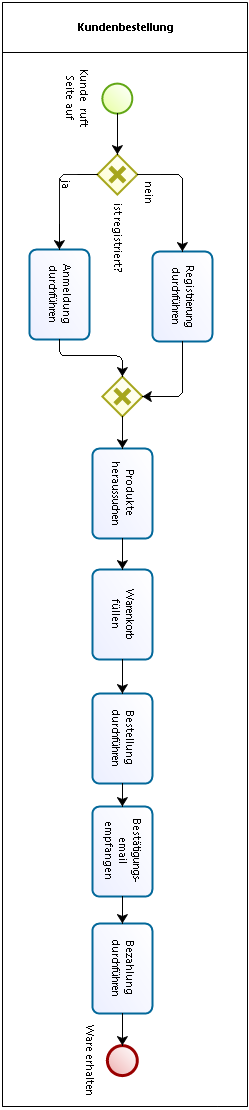
\includegraphics[width=50mm]{Bilder/Abbildung1-Geschaeftsprozess.png}
  \caption{Geschäftsprozess des Webshops}
  \label{fig:Abbildung 1}
\end{figure}


\subsection{Risikoanalyse$^2$}

Ein wichtiger Bestandteil der Projektplanung ist die Risikoanalyse. Sie umfasst alle ermittelten Risiken, die zur Laufzeit des Projekts auftrete können und entsprechende Gegenmaßnahmen. Um die Risiken zu ermitteln wurde zuvor eine Risikoanalyse durchgeführt. Bei der Risikoanalyse werden die Risiken hinsichtlich ihrer Tragweite und Wahrscheinlichkeit bewertet. Die Bewertung reicht dabei von gering, über eher gering, eher hoch bis hoch. \textit{Abbildung 2} zeigt die Einstufungen der Risiken zum Projekt sowie entsprechende Gegenmaßnahmen:

\begin{figure}[H] 
  \centering
     \fbox {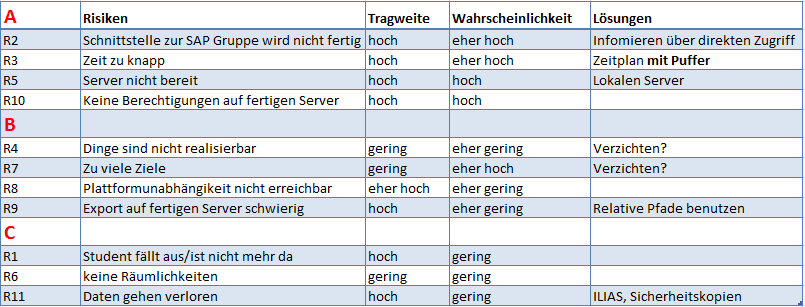
\includegraphics[width=15cm]{Bilder/Risikoanalyse1.png}}
  \caption{Einstufung der Risiken und entsprechende Gegenmaßnahmen}
  \label{fig:Abbildung 2}
\end{figure}

Die Risiken werden in drei Kategorien unterteilt. Kategorie A beschreibt Risiken, die eine hohe Tragweite und Wahrscheinlichkeit aufweisen. Kategorie B beschreibt Risiken, deren Tragweite und Wahrscheinlichkeit weder zu hoch noch zu gering eingestuft wurden. Kategorie C beschreibt Risiken, deren Tragweite und Wahrscheinlichkeit eher gering eingestuft wurden.

Der Kategorie A wurden die Risiken „SAP-Gruppe wird nicht mit Datenbank fertig“, „Zeit zu knapp“, „Server nicht bereit“ und „Keine Berechtigungen auf fertigen Server“ hinzugefügt.  Das Risiko des Zeitmangels ist bei den meisten Projekten das größte Problem. Mangelnde Zeit bedeutet, dass das Projekt nicht im vollen Umfang fertiggestellt werden kann. Daher wurde es als eines der höchsten Risiken eingestuft. Risiken im Zusammenhang mit dem Server fallen ebenfalls unter dieser Kategorie. Ohne einen Server kann die Seite nicht betrieben werden, weshalb dieser kontinuierlich zur Verfügung stehen muss. Die SAP-Gruppe ist die wichtigste Schnittstelle, die es zu beachten gilt, da diese die Datenbank für den Webshop zur Verfügung stellt. Ohne Datenbank ist der Webshop nicht voll funktionsfähig.
\\
Der Kategorie B wurden die Risiken „Dinge sind nicht realisierbar“, „Zu viele Ziele“, „Plattformunabhängigkeit nicht erreichbar“ und „Export auf fertigen Server schwierig“ hinzugefügt. Wenn sich bei den Zielen eines Projekts verschätzt wird und dadurch zu viele oder unrealistische Ziele gesetzt werden, kann nicht der vorher vereinbarte Umfang des Projekts gewährleistet werden. Plattformunabhängigkeit ist eines der vereinbarten Anforderungen. Der Webshop sollte auf jeden Browser dargestellt werden können. Je mehr Browser die Webseite unterstützt, desto mehr Kunden können angesprochen werden. Der Export auf den fertigen Server könnte sich als schwierig erweisen, wenn Programme, die für den Export benötigt werden, nicht auf dem Server vorhanden sind.
\\
Der Kategorie C wurden die Risiken „Student fällt aus/ist nicht mehr da“, „keine Räumlichkeiten vorhanden“ und „Daten gehen verloren“ hinzugefügt. Diese Risiken können auftreten, sind aber für das Projekt keine große Bedrohung. Das Risiko eines Datenverlustes wird durch mehrere Backups stark gemindert.
\\
Das Risiko „Student fällt aus/ist nicht mehr da“ wurde anfangs als gering eingestuft.  Zum jetzigen Zeitpunkt wird dieses Risiko allerdings als hoch eingestuft, da die Gruppenmitglieder Herr Gregarek und Herr Dück schon mehrfach ausgefallen sind.
\\
\textit{Abbildung 3} zeigt die Ergebnisse der Risikoanalyse anhand einer Grafik:

\begin{figure}[H] 
  \centering
     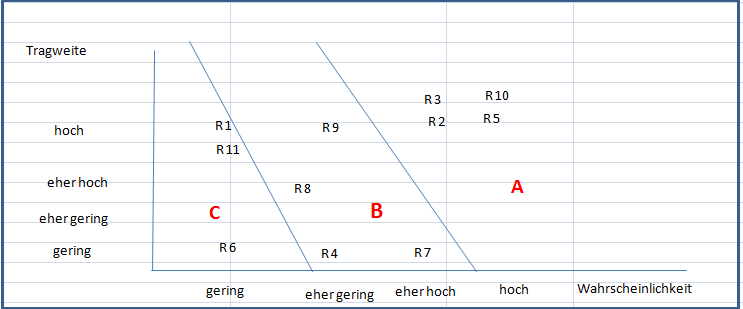
\includegraphics[width=15cm]{Bilder/Risikoanalyse2.png}
  \caption{Ergebnisse der Risikoanalyse}
  \label{fig:Abbildung 3}
\end{figure}

Dabei lässt sich die Einteilung der Risiken in den einzelnen Kategorien besser nachvollziehen.

\subsection{Wahl der Programmiersprache$^1$}
Nachdem die Anforderungen an das Projekt festgelegt waren, wurde sich mit der Festlegung der Programmiersprache beschäftigt. Es stand Java Enterprise Edition und PHP zur Auswahl. Die Auswahl viel auf PHP, da aus alten Projekten und der Webdesign-Vorlesung schon Vorwissen über die Programmierung von Webseiten in PHP vorhanden war. Zudem war auch geplant Teile des Quellcodes der alten Projekte für das neue Projekt wieder zu verwenden.

\subsection{Wahl der Programmierentwicklungsumgebung und des Versions-verwaltungs-Plugin$^1$}
Zu Beginn des Projekts hatte jedes Gruppenmitglied einen eigenen Texteditor und an einer eigenen Version des Projekts gearbeitet. Es fiel nach kurzer Zeit auf, dass so das Zusammenfügen der verschiedenen Versionen sehr aufwendig war. Aus diesen Grund wurde nach einer Möglichkeit gesucht, das Problem zu lösen. Es wurde das \glqq GitHub-Plugin\grqq{} für das Programm \glqq Eclipse\grqq{} als Lösung für das Versionsproblem gefunden. \\
Als Entwicklungsumgebung wurde sich für Eclipse entschlossen, da es bei installierten PHP-Plugin eine gute Autovervollständigung für PHP bietet. Zudem ist es als Portable-Version erhältlich und kann somit ohne Installation auf den Hochschulrechnern betrieben werden. \\
Als Versionsverwaltungssystem wurde sich für \glqq GitHub\grqq{} entschlossen, da dieses schon in den Programm \glqq Eclipse\grqq{} integriert ist. Zudem ist „GitHub“ eine Cloud basierte Lösung, welche das gemeinsame Arbeiten an einen Projekt ermöglicht. Das komplette Projekt wird dabei auf einen Server hochgeladen. Jedes Gruppenmitglied, das einen Account bei „GitHub“ erstellt hat, kann dem Projekt beitreten, indem es bei den Gruppen-Administrator um Erlaubnis bittet. Dadurch kann ein Dokument von mehreren Gruppenmitgliedern gemeinsam bearbeitet werden. So entstehen mehrere Versionen von einem Dokument, die anschließend wieder mit Hilfe eines in GitHub enthaltenden \glqq Merge-Tools\grqq{} zu einer gemeinsamen Version zusammengefügt werden können.


\subsection{Grundlegender Aufbau und Ordnerstruktur der Webseite$^1$}
Einer der ersten Schritte der praktischen Umsetzung des Projekts war die Festlegung der Ordnerstruktur der Webseite. Die Ordnerstruktur sollte einen einheitlichen Aufbau der Webseite garantieren. Mit der Festlegung sollte für jedes Projektmitglied definiert werden, wo welche Dateien abgelegt werden sollen und wie generell die programmiertechnische Struktur des Programms aussehen soll.  \\
Als Programmieransatz für das Projekt wurde die objektorientierte Programmierung gewählt. Die Hauptgründe für die Auswahl des Programmieransatzes waren, dass die objektorientierte Programmierung durch die Vererbung die Möglichkeit bietet schon programmierte Funktionen an andere Klassen zu übernehmen. Es wird also Programmierarbeit eingespart. Ein Beispiel für die Einsparung von Programmierarbeit ist, wenn ein Fehler in einer vererbten Methode ist, muss der Fehler nur bei der Eltern-Klasse behoben werden und nicht bei der Kind-Klasse. Ein weiterer Grund ist, dass die objektorientierte Programmierung auch die Übersichtlichkeit der Webseite fördert. Für jedes Objekt der Webseite wird einfach eine Klasse angelegt, welche dieses definiert. So wird z.B. eine Klasse für den Kunden oder den Warenkorb erstellt. Diese Klasse arbeitet alle Aufgaben des Objekts ab. Der letzte Grund für den Ansatz war, dass schon objektorientierte Quellcodes aus alten Projekten zur Verfügung standen. \\
Da sich für die objektorientierte Programmierung entschieden wurde, hat sich die Gruppe auf folgende Ordnerstruktur geeinigt:
\begin{figure}[H]
  \centering
     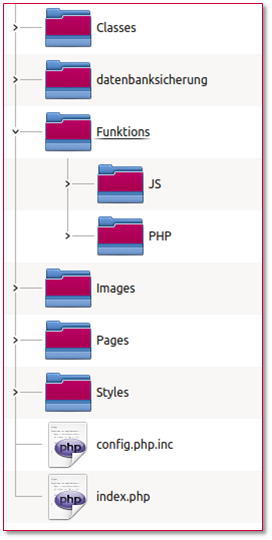
\includegraphics[width=45mm]{Bilder/ordnerstruktur.png}
  \caption{Ordnerstruktur des Projekts}
  \label{fig:Abbildung 4}
\end{figure}
Der Ordner \glqq Classes\grqq{} beinhaltet alle PHP-Klassen des Projekts. Dieser Ordner enthält zum Beispiel Klassen zur Umsetzung des Warenkorbs, des Datenbankzugriffs, des Kundens, der Kundenbestellung und so weiter. Der Ordner \glqq datenbanksicherung\grqq{} enthält die jeweils aktuelle Sicherung der Datenbank. Der folgende Ordner ist in zwei Unterordner aufgeteilt. Dieser Ordner wurde mit dem Namen \glqq Funktions\grqq{} bezeichnet. Der erste Unterordner, der den Namen \glqq JS\grqq{} trägt, enthält die clientseitig programmierten Funktionen. Die clientseitige Programmierung sollte in JavaScript umgesetzt werden. Aus diesen Grund sind in diesen Ordner JavaScript-Dateien vorzufinden. Die JavaScripts werden unter anderen dafür verwendet eine Formulareingabe vor den Absenden auf Gültigkeit zu überprüfen. Dieses sorgt dafür, dass es nicht zu unnötigen Datenverkehr zwischen Browser und Webserver kommt. Der Unterordner \glqq PHP\grqq{} enthält die Funktionen, die zum Beispiel nach dem Absenden einer Formulareingabe an den Webserver aufgerufen werden. Diese Funktionen instanzieren die Klassen. Zudem rufen die Funktionen-Dateien die entsprechenden Methoden auf, um die vom Formular empfangenen Eingaben zu verarbeiten. Dieser Ordner enthält noch zwei weitere Dateien. Die erste der beiden Dateien heißt \glqq set\_page.php.inc\grqq{}. Diese Datei ließt einen über die Adressenzeile erhaltenden Parameter aus. Anhand des Parameters bestimmt die Datei, welcher Inhalt aktuell auf der Webseite angezeigt werden soll. Hierzu inkludiert die Datei die entsprechende HTML-Seite aus dem Ordner \glqq Pages\grqq{}. Die zweite Datei heißt \glqq  set\_control.php.inc\grqq{}. Diese Datei inkludiert die benötigte Funktions-Datei, die z.B. die Formulareingaben bearbeiten. \\
In diesem Projekt werden keine in PHP programmierten Funktionen und Inhaltseiten direkt aufgerufen. Diese Dateien werden immer in die Index.php inkludiert. Der Grund hierfür ist, dass so dem Anwender der interne Aufbau der Webseite verborgen bleibt.\\
Der Ordner \glqq Images\grqq{} enthält die Bilder, die auf der Webseite angezeigt werden. Der letzte Ordner mit dem Namen \glqq Styles\grqq{} enthält die CSS-Dateien, die das Design der Webseite festlegen. In der \glqq config.php.inc\grqq{}-Datei werden grundlegende Konfigurationen für den Webshop festgelegt. In dieser Datei sind unter anderen die Zugangsdaten für die Datenbank angegeben. Die \glqq index.php\grqq{} ist die standardmäßige Webseiteneinstiegsdatei. Über diese Datei wird die Webseite geladen.

\subsection{Die Test-Server$^1$}
Um bei der Entwicklung nicht erst darauf warten zu müssen bis die Server-Gruppe die benötigten Server-Dienst aufgesetzt hat, wurde sich nach eine Möglichkeit umgesehen, wie man für Testzwecke die Webseite auf den Hochschulrechnern laufen lassen könnte. Hierfür wurde das Programm XAMPP gefunden. Es ist eine Software-Sammlung, die alle benötigten Server-Dienste für PHP-Webseiten auf einen Windows-Rechner bereitstellt. Die Softwaresammlung bietet den Vorteil, dass eine portable Version erhältlich ist. Diese Version kann ohne Administrationsrechte ausgeführt werden.

\subsection{Zeitplan$^2$}
Nachfolgend wird der Zeitplan des Projekts dargestellt. Für jedes Arbeitspaket wurde eine Zeit von zwei Wochen eingeplant. Da jedes Gruppenmitglied 3 Arbeitspakte zugeteilt bekam, betrug die reine Arbeitszeit 6 Wochen. Herr Schnürer und Herr Brüntrup konnte diese Zeit weitestgehend einhalten. Zu der Arbeitszeit von Herrn Gregarek und Herrn Dück  ist nichts Näheres bekannt. Da deren Arbeitspakte jedoch nicht vollständig bearbeitet wurden, ist deren Arbeitszeit deutlich geringer einzuschätzen. Die Arbeitszeit von 6 Wochen trug dazu bei, dass die Sommersemesterferien als Pufferzeit eingeplant werden konnten. \textit{Abbildung 5} zeigt den Zeitplan, während \textit{Abbildung 6} das dazugehörige Gantt-Diagramm zeigt. \textit{Abbildung 7-10} beschreiben den aktuellen Projektstand vom 07. August 2015 anhand eines Ampelsystems. 

\begin{figure}[H] 
  \centering
     \fbox{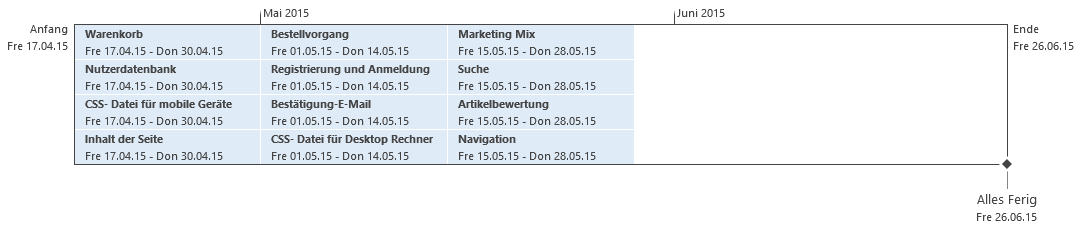
\includegraphics[width=160mm]{Bilder/Abbildung16_Zeitplan.png}}
  \caption{Zeitplan}
\end{figure}

\begin{figure}[H] 
  \centering
     \fbox{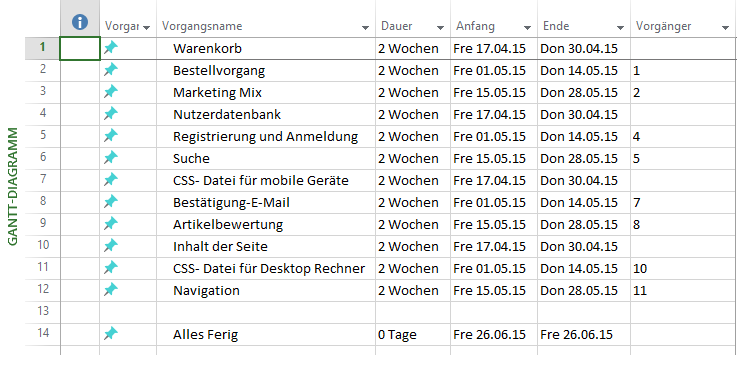
\includegraphics[width=15cm]{Bilder/Abbildung17_GanttDiagramm.png}}
  \caption{Zeitplan}
\end{figure}

\begin{figure}[H] 
  \centering
  \fbox{
     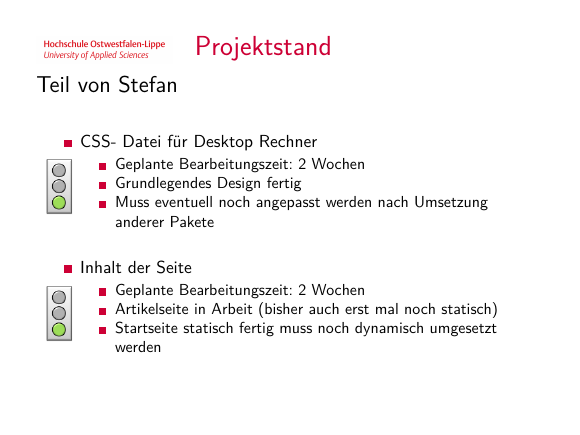
\includegraphics[width=10cm]{Bilder/projektstand1.png}}
  \caption{Zeitplan}
\end{figure}


\begin{figure}[H] 
  \centering
  \fbox{
     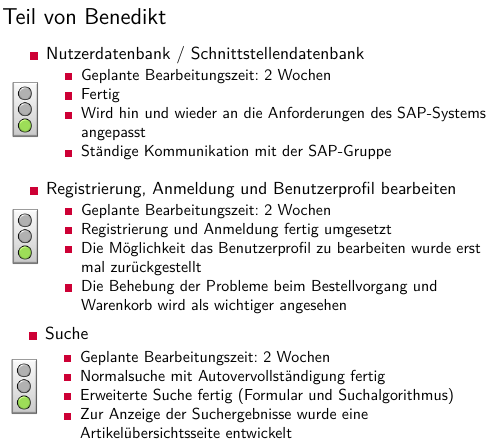
\includegraphics[width=10cm]{Bilder/projektstand3.png}}
  \caption{Zeitplan}
\end{figure}


\begin{figure}[H] 
  \centering
  \fbox{
     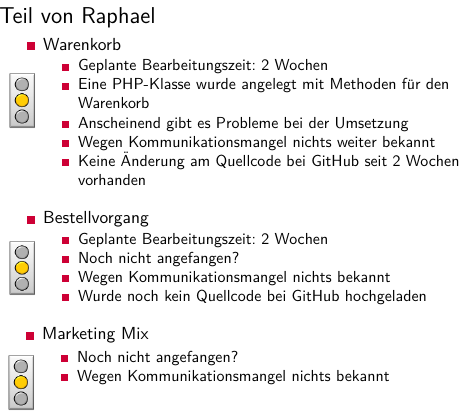
\includegraphics[width=10cm]{Bilder/projektstand5.png}}
  \caption{Zeitplan}
\end{figure}


\begin{figure}[H] 
  \centering
  \fbox{
     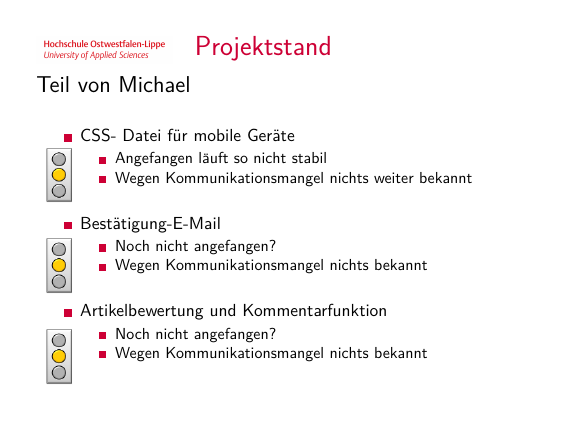
\includegraphics[width=10cm]{Bilder/projektstand7.png}}
  \caption{Zeitplan}
\end{figure}

